\chapter{Variaciones del Modelo}\label{chap:variaciones}

Teniendo ya claros los conceptos médicos y el análisis de un modelo base acorde con tales conceptos, es momento de introducir al modelo las dos enfermedades presentadas en \ref{sec:RBC:enfermedades}. El caso de las hemorragias es más sencillo que el de la anemia, pues los sangrados son tratados una única vez (hasta que sean frenados), mientras que la anemia es una enfermedad cuyo tratamiento es para toda la vida. En este capítulo se presentarán las variaciones matemáticas del modelo y el análisis de las simulaciones de estas, esperando que los resultados obtenidos logren mantener la homeostasis del paciente y, para el caso de la anemia, ver si un aumento o disminución de la dosis afecta realmente los resultados.

\section{Caso con Hemorragia}\label{Sec:variaciones:hemorragia}

Para los sangrados, se tendrán en cuenta diferentes casos. Inicialmente se tendrá en cuenta una hemorragia leve (pérdida del 2$\%$ de sangre) y se observará lo que sucede si, después de la pérdida de sangre, las variables del modelo se mantienen iguales y que sucede si estas se modifican. Posteriormente se considerará el caso de una hemorragia grave (el 14$\%$ de la sangre del cuerpo) y se observarán los efectos de una transfusión sanguínea para recuperar la homeostasis. En el caso de las hemorragias, se tendrá en cuenta el caso en el que $\gamma =1$, pues así el paciente es totalmente sano, el parámetro $f$ se mantiene igual que antes ($=0.00832$) y los valores iniciales también se mantienen.

\subsection{Hemorragia Leve}\label{subsec:variaciones:hemorragia:leve}

Para esta variación del modelo, considere que en el tercer día de medición el paciente, ya sea por un corte o un accidente, pierde el $2\%$ de su cantidad de sangre en el cuerpo que, considerando el caso de que tenga 5 litros de sangre, esto equivale a 100 mililitros de fluido o a $5\times 10^{11}$ glóbulos rojos. Así, el modelo se puede ver de la siguiente manera:

$$R(n+1)= \left\{ \begin{array}{lcc} (1-f)\cdot R(n)+M(n) & \textrm{si} & n \neq 3 \\ \\ (1-f)\cdot R(n)+M(n)-0.02\cdot R(n) & \textrm{si} & n = 3\end{array} \right.$$

$$M(n+1)=\gamma \cdot f \cdot R(n)$$

En donde:
\begin{itemize}
    \item $\gamma=1$;
    \item $f=0.00832$;
    \item $R(0) = 25\times 10^{12};$
    \item $M(0) = 208 \times 10^{9}.$
\end{itemize}

Así, la simulación se ve así: en la primera gráfica de la figura \ref{sec:variaciones:fig:HemoLeveG1} se observa la pérdida de RBC's en el tercer día, un aumento del tercero al cuarto y estabilidad del cuarto en adelante. En la segunda gráfica se observa lo mismo pero con un día de atraso. El aumento que se puede observar está dado por el hecho de que el adendo $M(n)$ conserva lo que ha ocurrido en $R(n-1)$ así, para el cuarto día se producen la cantidad de eritrocitos que se vienen produciendo regularmente antes del accidente, y desde el cuarto día en adelante este adendo ya se acomoda a la nueva cantidad de sangre. La estabilidad que se observa del cuarto día en adelante está dada por el hecho de que $\gamma = 1$, el modelo, de esta manera, funciona como lo hace normalmente (véase \ref{subsec:modelo:simulaciones:G1}) tomando una cantidad inicial de sangre menor que la original, es decir que mantiene una estabilidad con la cantidad de RBC's del cuarto día, que es de $24.504\times 10^{12}$ glóbulos rojos. 

\begin{figure}[H]
    \centering
    \captionsetup{justification=centering}
    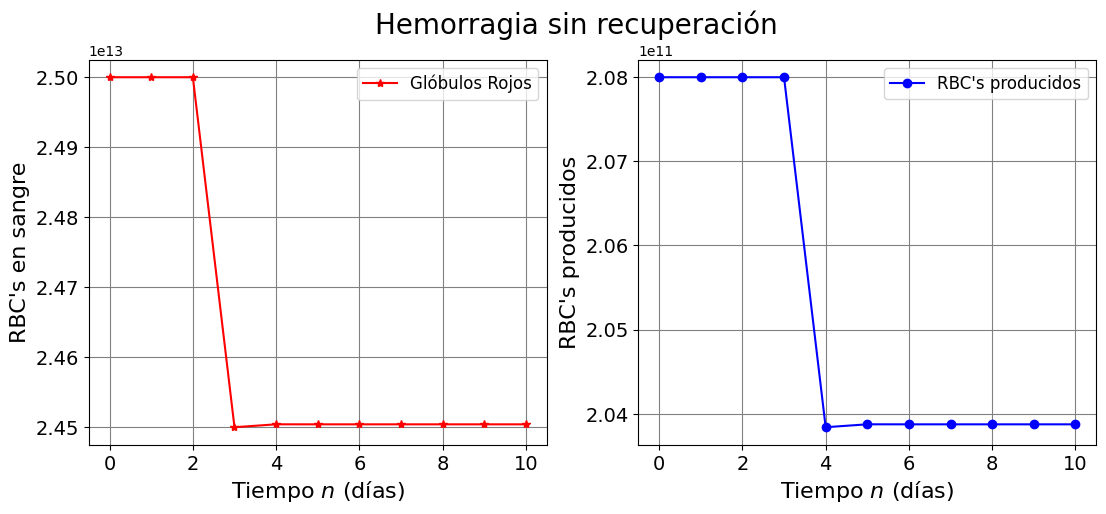
\includegraphics[scale=0.534]{figures/HemoLeveG1.png}
    \caption{Simulación del modelo para el caso de una hemorragia sin recuperación de la homeostasis. A la izquierda está la gráfica de $R(n)$, a la derecha la de $M(n)$.}
    \label{sec:variaciones:fig:HemoLeveG1}
\end{figure}

Está claro que esta simulación está totalmente alejada de lo que ocurre en el caso real, pues lo esperado es que el cuerpo recupere con el paso del tiempo la cantidad de glóbulos rojos perdidos, esto quiere decir que para $n>3$ se debe aumentar el valor de $\gamma$ hasta que la cantidad de eritrocitos sea mayor o igual a la inicial, es decir:

$$R(n+1)= \left\{ \begin{array}{lcc} (1-f)\cdot R(n)+M(n) & \textrm{si} & n \neq 3 \\ \\ (1-f)\cdot R(n)+M(n)-0.02\cdot R(n) & \textrm{si} & n = 3\end{array} \right.$$

$$M(n+1)=\left\{ \begin{array}{lcc} f\cdot \gamma_1 \cdot R(n) & \textrm{si} & R(n+1) \geq R(0) \\ \\ f\cdot \gamma_2\cdot R(n) & \textrm{si} & R(n+1)<R(0)\end{array} \right.$$

En donde:
\begin{itemize}
    \item $\gamma_1=1$;
    \item $\gamma_2=1.305$
    \item $f=0.00832$;
    \item $R(0) = 25\times 10^{12};$
    \item $M(0) = 208 \times 10^{9}.$
\end{itemize}

La condición de $M(n+1)$ permite evitar el retraso del que se ha hablado anteriormente, pues si se considera que ya se alcanzó la cantidad "normal" de eritrocitos entonces el cuerpo no debe producir más de los necesarios.

Para estimar el valor de $\gamma_2$ se utilizó la información brindada por el hospital general de Massachusetts en \cite{Massachusetts}, dado que al cuerpo le toma recuperar los glóbulos rojos perdidos en 450 ml de sangre en unas 5 semanas (35 días), entonces 100 ml deben recuperarse en unos 8 días. Las simulaciones hechas muestran que $\gamma=1.305$ permite lograr esta recuperación en ese tiempo.

Para estas simulaciones, se utilizó un tiempo de 15 días para poder observar lo que sucede después de recuperar los eritrocitos perdidos:

\begin{figure}[H]
    \centering
    \captionsetup{justification=centering}
    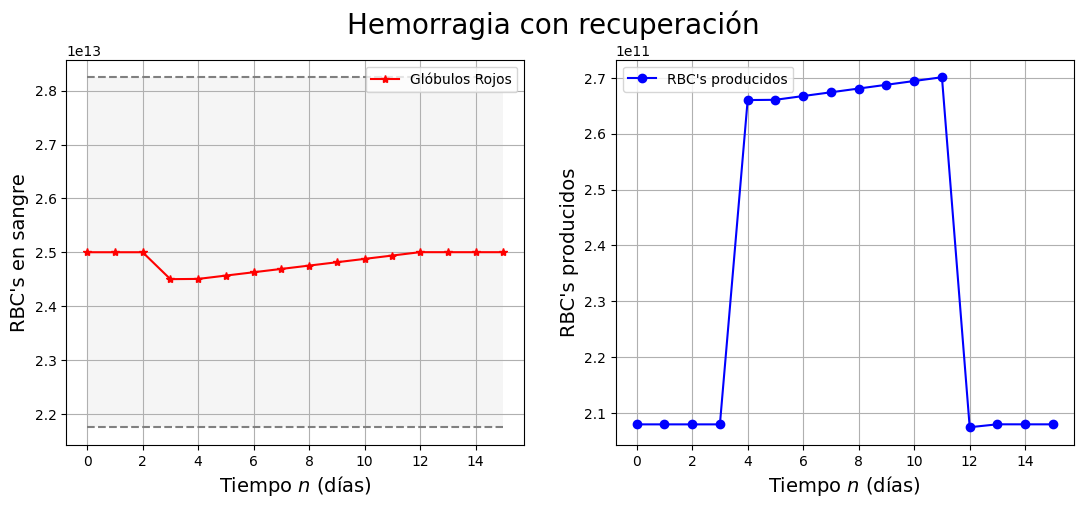
\includegraphics[scale=0.534]{figures/HemoLeveG13.png}
    \caption{Simulación del modelo para el caso de una hemorragia con recuperación de la homeostasis. A la izquierda está la gráfica de $R(n)$, a la derecha la de $M(n)$.}
    \label{sec:variaciones:fig:HemoLeveG13}
\end{figure}

Lo que se puede ver en estas gráficas es como, a partir del cuarto día (dado el retraso que presenta el modelo) se hace efectivo el cambio de $\gamma_1$ a $\gamma_2$, que se evidencia por el aumento en la primera gráfica de la figura \ref{sec:variaciones:fig:HemoLeveG13} del cuarto al duodécimo día y en la segunda gráfica del cuarto al undécimo día. En el día 12 es en el que por fin se ha superado (o igualado) la cantidad inicial de glóbulos rojos en el cuerpo, el aumento desde la pérdida muestra lo ilustrado en la sección \ref{subsec:modelo:simulaciones:G13}, donde hay un aumento constante de eritrocitos. Después de recuperar la cantidad de sangre perdida, el cuerpo vuelve a estabilizar su sistema, pues ha llegado a la homeostasis. La diferencia en la segunda gráfica de los días 0 a 3 y de los días 13 a 15 se debe a que ha aumentado la cantidad estable de sangre, y para compensar la pérdida el cuerpo debe producir más células.

Teniendo esto en cuenta, ahora se debe analizar el caso en el que el paciente sufre de una hemorragia más grave y debe ser sometido a una transfusión sanguínea para que pueda recuperarse.

\subsection{Hemorragia Grave}

Considérese el caso en el que el paciente analizado sufre una pérdida del 14$\%$ del volumen de sangre de su cuerpo (unos 700 mililitros o 3.25$\times 10^{12}$ eritrocitos) a causa de un accidente, ya sea una hemorragia interna causada por un golpe o una herida externa como un corte. Esta pérdida de sangre es cercana al 20$\%$ que se puede considerar fatal, por lo que la pérdida de sangre presentada se puede considerar como grave y debe ser tratada médicamente mediante una transfusión sanguínea.

Dado que las bolsas de transfusión de glóbulos rojos tienen un volumen aproximado de 250 mililitros (el 5$\%$ de la concentración normal, unos 1.25$\times 10^{12}$ RBC's), entonces para subsanar la pérdida se le suministrarán dos bolsas de eritrocitos y el volumen restante podrá ser recuperado por el cuerpo.

Para poder adecuar el problema al modelo, se considerará que el sangrado inicia y termina en el tercer día y el suministro de sangre ocurre y finaliza en el cuarto. Esta situación no es muy realista, pues en una complicación médica se debe tratar el problema lo más rápido posible, pero para esta investigación es util definir este caso de tal manera para poder ilustrar correctamente las ecuaciones. Es importante notar que el cuerpo tendrá cuatro estados durante este caso: la estabilidad antes y después de la recuperación, el día en el que se hace la transfusión y los días después de la transfusión. De esta manera, el cuerpo debe modificar su producción interna de RBC's en tres momentos, generando dos valores nuevos de $\gamma$.

Así, una hemorragia grave se puede interpretar con la siguiente modificación del modelo base:

$$R(n+1)= \left\{ \begin{array}{lcc} (1-f)\cdot R(n)+M(n) & \textrm{si} & n \neq 3,4 \\ \\ (1-f)\cdot R(n)+M(n)-0.02\cdot R(n) & \textrm{si} & n = 3 \\ \\ (1-f)\cdot R(n)+M(n)+0.1\cdot R(0) & \textrm{si} & n = 4 \\ \end{array} \right.$$

$$M(n+1)=\left\{ \begin{array}{lcc} f\cdot \gamma_1 \cdot R(n) & \textrm{si} & R(n+1) \geq R(0) \\ \\ f\cdot \gamma_2\cdot R(n) & \textrm{si} & n = 4 \\ \\ f\cdot \gamma_3\cdot R(n) & \textrm{si} & n \neq 4\textrm{ y } R(n+1)<R(0)\\ \end{array} \right.$$

En donde:
\begin{itemize}
    \item $\gamma_1=1$;
    \item $\gamma_2=1.331$;
    \item $\gamma_3=1.31$;
    \item $f=0.00832$;
    \item $R(0) = 25\times 10^{12};$
    \item $M(0) = 208 \times 10^{9}.$
\end{itemize}
Los valores de $\gamma_2$, $\gamma_3$ fueron estimados al igual que en el caso de hemorragias leves. La cantidad de glóbulos rojos perdida en 700 mililitros de sangre debería ser recuperada por el cuerpo en unos 55 días, obteniendo un valor de $\gamma_2$ de 1.331. Para estimar $\gamma_3$ se debe tener en cuenta la cantidad de eritrocitos en el cuerpo en el quinto día, pues el cuerpo del paciente se ajusta a la nueva cantidad de glóbulos rojos obtenidos gracias a la transfusión. En el quinto día de simulación, el cuerpo tiene 24.0673$\times 10^{12}$ RBC's, siguiendo la cuenta del hospital general de Massachusetts, la cantidad restante (93.2713 $\times 10^{10}$ eritrocitos) se recuperaría en 15 días, es decir que $\gamma_3 = 1.31$ según las simulaciones del modelo.

Para ilustrar los diferentes estados del cuerpo mencionados anteriormente, se amplió el tiempo de simulación a 22 días: 

\begin{figure}[H]
    \centering
    \captionsetup{justification=centering}
    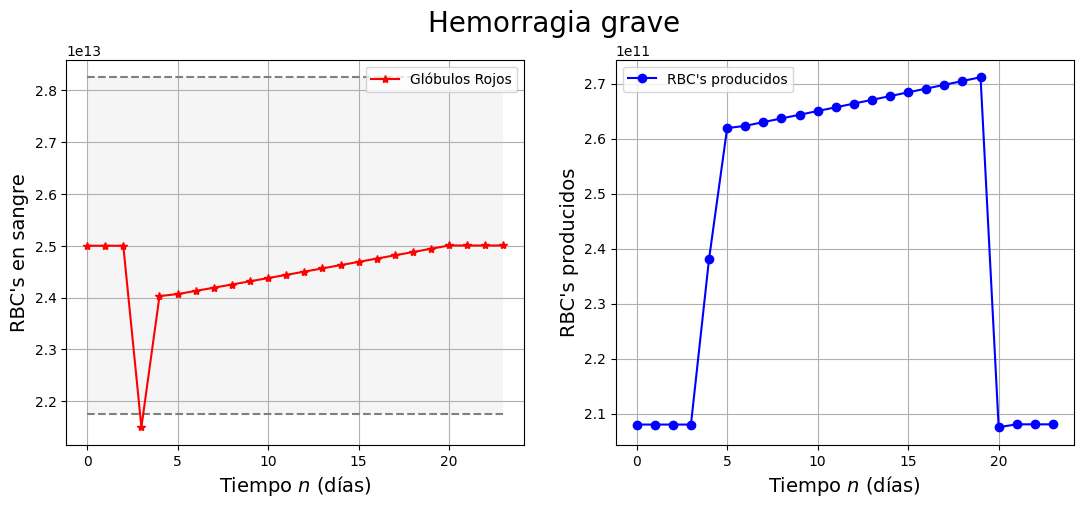
\includegraphics[scale=0.534]{figures/HemoGrave.png}
    \caption{Simulación del modelo para el caso de una hemorragia grave con transfusión. A la izquierda está la gráfica de $R(n)$, a la derecha la de $M(n)$.}
    \label{sec:variaciones:fig:HemoLeveG13}
\end{figure}